
%(BEGIN_QUESTION)
% Copyright 2006, Tony R. Kuphaldt, released under the Creative Commons Attribution License (v 1.0)
% This means you may do almost anything with this work of mine, so long as you give me proper credit

Complete the following ladder-logic schematic diagram for part of a cooling water reservoir level control system, inserting the correct types of level switches in the correct locations, complete with all necessary interconnecting wires:

$$\includegraphics[width=15.5cm]{i00515x01.eps}$$

One level switch, set at 3 feet, controls the low water level warning lamp, energizing the lamp if the water level ever drops below 3 feet in the reservoir.  Another level switch, set at 2 feet, controls the utility water make-up valve, opening this valve to add more water from the clean water supply to the reservoir if the reservoir level ever drops below 2 feet.  The final level switch is set at 5 feet, and controls the high water level warning lamp, energizing the lamp if the water level ever rises above 5 feet in the reservoir.

\vskip 10pt

\noindent
Credit will be given for correctly wiring each of the three branch circuits.  You {\it must} write the given level setting (in feet) next to each switch in order to receive credit for that circuit:

\begin{itemize}
\item{} Low water level warning lamp
\item{} Make-up water solenoid valve
\item{} High water level warning lamp
\end{itemize}

\underbar{file i00515}
%(END_QUESTION)





%(BEGIN_ANSWER)

$$\includegraphics[width=15.5cm]{i00515x02.eps}$$

3 points for each warning lamp switch, 4 points for solenoid valve switch.

%(END_ANSWER)





%(BEGIN_NOTES)

{\bf This question is intended for exams only and not worksheets!}.

%(END_NOTES)


